\documentclass{article}
\newcommand\tab[1][1cm]{\hspace*{#1}}
\usepackage[english]{babel}
\usepackage{multicol}
\usepackage[utf8]{inputenc}
\usepackage{tikz}\usetikzlibrary{arrows,automata}
\usepackage{graphicx}
\usepackage{grffile}

\usepackage{fancyhdr}
\usepackage{enumerate}
\usepackage{amsmath}
\usepackage{amsfonts}
\usepackage{amssymb}

\title{Algorithms - CS:344 - Midterm 2 Study Guide}
\begin{document}
\maketitle{}
\section*{DFS}

	The \textbf{General Approach} to applying \textit{Depth First Search} is to pick a starting state and mark the node as visted. Next, recursivley step to the first neighbor from the list of neighbors that is stored within the first vertex. Mark this new node as visted and repeat the process for all $N$ first neighbors or until we reach a node that has already been visited. Once all the first neighbors have been visited, go back one vertex from the previous recursive iteration check the second Neighbor of said vertex. Repeat this process until the vertex you are checking has been seen, and or you reach a node that has no other neighbors. Repeat the process from step 1 and 2 on all nodes until every node has been seen. \\ \\
	\begin{minipage}{.4\textwidth}
		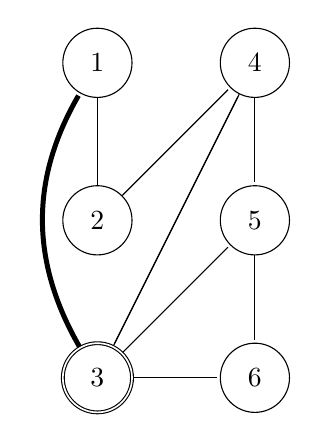
\begin{tikzpicture}[>=stealth',shorten >=1pt,auto,node distance=2cm]
                  \node[state]  	      (1) []           {$1$};
                  \node[state]            (2) [below of=1] {$2$};
                  \node[state, accepting] (3) [below of=2] {$3$};
                  \node[state] 			  (4) [right of=1] {$4$};
                  \node[state]		 	  (5) [right of=2] {$5$};
                  \node[state]		 	  (6) [right of=3] {$6$};

                      \draw[-, line width = 1.8pt] 
                               (3) edge [bend left](1)
                                   edge [thin] (4)
                                   edge [thin] (5)
                                   edge [thin] (6)
                               (2) edge [thin] (1)
                                   edge [thin] (4)
                               (1) edge [thin] (2)
                               (4) edge [thin] (5)
                                   edge [thin] (3)
                               (5) edge [thin] (6);       	 		
		\end{tikzpicture}
	\end{minipage}
	\begin{minipage}{.4\textwidth}
		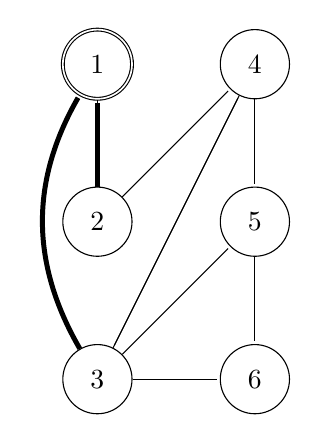
\begin{tikzpicture}[>=stealth',shorten >=1pt,auto,node distance=2cm]
                \node[state, accepting] (1) []           {$1$};
                \node[state]            (2) [below of=1] {$2$};
                \node[state]  			(3) [below of=2] {$3$};
                \node[state] 			(4) [right of=1] {$4$};
                \node[state]		 	(5) [right of=2] {$5$};
                \node[state]		 	(6) [right of=3] {$6$};

                    \draw[-, line width = 1.8pt] 
                             (3) edge [bend left](1)
                                 edge [thin] (4)
                                 edge [thin] (5)
                                 edge [thin] (6)
                             (2) edge (1)
                                 edge [thin] (4)
                             (1) edge [thin] (2)
                             (4) edge [thin] (5)
                                 edge [thin] (3)
                             (5) edge [thin] (6);       	 		
		\end{tikzpicture}
    \end{minipage}
    \begin{minipage}{.4\textwidth}
        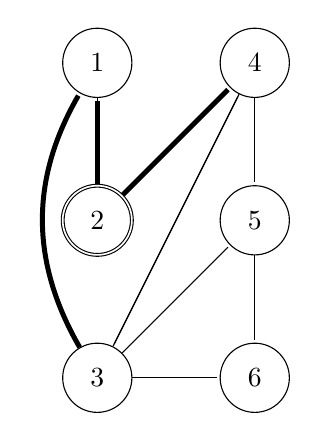
\begin{tikzpicture}[>=stealth',shorten >=1pt,auto,node distance=2cm]
                  \node[state]  			(1) []           {$1$};
                  \node[state, accepting]	(2) [below of=1] {$2$};
                  \node[state] 				(3) [below of=2] {$3$};
                  \node[state] 				(4) [right of=1] {$4$};
                  \node[state]		 		(5) [right of=2] {$5$};
                  \node[state]		 		(6) [right of=3] {$6$};

                      \draw[-, line width = 1.8pt] 
                               (3) edge [bend left](1)
                                   edge [thin] (4)
                                   edge [thin] (5)
                                   edge [thin] (6)
                               (2) edge (1)
                                   edge (4)
                               (1) edge [thin] (2)
                               (4) edge [thin] (5)
                                   edge [thin] (3)
                               (5) edge [thin] (6);       	 		
        \end{tikzpicture}
    \end{minipage}
    \begin{minipage}{.4\textwidth}
        \vspace{\baselineskip}
        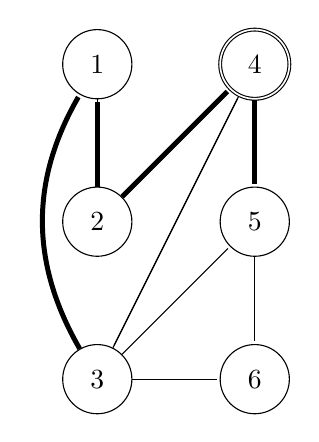
\begin{tikzpicture}[>=stealth',shorten >=1pt,auto,node distance=2cm]
                      \node[state]  		(1) []           {$1$};
                      \node[state]          (2) [below of=1] {$2$};
                      \node[state] 			(3) [below of=2] {$3$};
                      \node[state,accepting](4) [right of=1] {$4$};
                      \node[state]		 	(5) [right of=2] {$5$};
                      \node[state]		 	(6) [right of=3] {$6$};

                          \draw[-, line width = 1.8pt] 
                                   (3) edge [bend left](1)
                                       edge [thin] (4)
                                       edge [thin] (5)
                                       edge [thin] (6)
                                   (2) edge (1)
                                       edge (4)
                                   (1) edge [thin] (2)
                                   (4) edge (5)
                                       edge [thin] (3)
                                   (5) edge [thin] (6);       	 		
          \end{tikzpicture}
    \end{minipage}
    \begin{minipage}{.4\textwidth}
        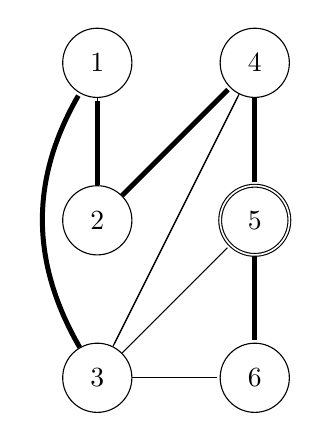
\begin{tikzpicture}[>=stealth',shorten >=1pt,auto,node distance=2cm]
                  \node[state]  		(1) []           {$1$};
                  \node[state]          (2) [below of=1] {$2$};
                  \node[state] 			(3) [below of=2] {$3$};
                  \node[state] 			(4) [right of=1] {$4$};
                  \node[state,accepting](5) [right of=2] {$5$};
                  \node[state]		 	(6) [right of=3] {$6$};

                      \draw[-, line width = 1.8pt] 
                               (3) edge [bend left](1)
                                   edge [thin] (4)
                                   edge [thin] (5)
                                   edge [thin] (6)
                               (2) edge (1)
                                   edge (4)
                               (1) edge [thin] (2)
                               (4) edge (5)
                                   edge [thin] (3)
                               (5) edge (6);       	 		
        \end{tikzpicture}
	\end{minipage}
    \begin{minipage}{.4\textwidth}
        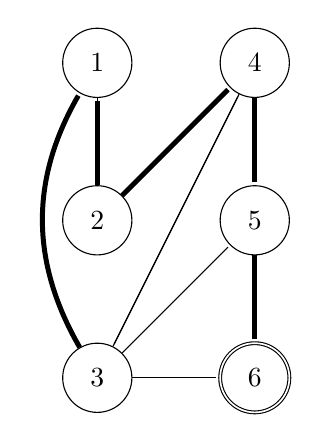
\begin{tikzpicture}[>=stealth',shorten >=1pt,auto,node distance=2cm]
                  \node[state]  		(1) []           {$1$};
                  \node[state]          (2) [below of=1] {$2$};
                  \node[state] 			(3) [below of=2] {$3$};
                  \node[state] 			(4) [right of=1] {$4$};
                  \node[state]			(5) [right of=2] {$5$};
                  \node[state,accepting](6) [right of=3] {$6$};

                      \draw[-, line width = 1.8pt] 
                               (3) edge [bend left](1)
                                   edge [thin] (4)
                                   edge [thin] (5)
                                   edge [thin] (6)
                               (2) edge (1)
                                   edge (4)
                               (1) edge [thin] (2)
                               (4) edge (5)
                                   edge [thin] (3)
                               (5) edge (6);       	 		
        \end{tikzpicture}
	\end{minipage}
 
\section*{BFS}

  
		
	The \textbf{General Algorithm} to Breadth First Search is to first look at a vertex and enqueue said vertex. From there, we mark that we visited said vertex and enqueue the neighboring unseen verticies. Repeat this process until the queue is empty.  
		
    	
    
    \begin{minipage}{.4\textwidth}
        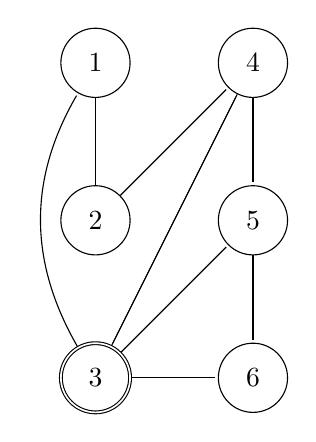
\begin{tikzpicture}[>=stealth',shorten >=1pt,auto,node distance=2cm]
                \node[state]  			(1) []           {$1$};
                \node[state]            (2) [below of=1] {$2$};
                \node[state, accepting] (3) [below of=2] {$3$};
                \node[state] 			(4) [right of=1] {$4$};
                \node[state]		 	(5) [right of=2] {$5$};
                \node[state]		 	(6) [right of=3] {$6$};

                    \path[-] (3) edge [bend left](1)
                                 edge (4)
                                 edge (5)
                                 edge (6)
                             (2) edge (1)
                                 edge (4)
                             (1) edge (2)
                             (4) edge (5)
                                 edge (3)
                             (5) edge (6);       	 		
            \end{tikzpicture}
	\end{minipage}
	\begin{minipage}{.4\textwidth}
        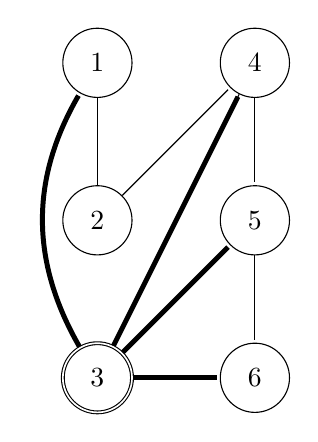
\begin{tikzpicture}[>=stealth',shorten >=1pt,auto,node distance=2cm]
            \node[state]  			(1) []           {$1$};
            \node[state]            (2) [below of=1] {$2$};
            \node[state, accepting] (3) [below of=2] {$3$};
            \node[state] 			(4) [right of=1] {$4$};
            \node[state]		 	(5) [right of=2] {$5$};
            \node[state]		 	(6) [right of=3] {$6$};

            	\draw[-, line width = 1.8pt] 
                		 (3) edge [bend left](1)
                             edge (4)
                             edge (5)
                             edge (6)
                         (2) edge [thin] (1)
                             edge [thin] (4)
                         (1) edge [thin] (2)
                         (4) edge [thin] (5)
                             edge [thin] (3)
                         (5) edge [thin] (6);       	 		
        \end{tikzpicture}
	\end{minipage}
	\begin{minipage}{.35\textwidth}
        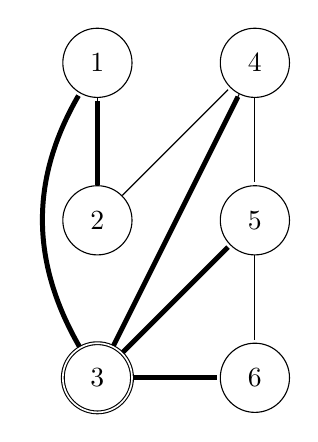
\begin{tikzpicture}[>=stealth',shorten >=1pt,auto,node distance=2cm]
            \node[state]  			(1) []           {$1$};
            \node[state]            (2) [below of=1] {$2$};
            \node[state, accepting] (3) [below of=2] {$3$};
            \node[state] 			(4) [right of=1] {$4$};
            \node[state]		 	(5) [right of=2] {$5$};
            \node[state]		 	(6) [right of=3] {$6$};

            	\draw[-, line width = 1.8pt] 
                		 (3) edge [bend left](1)
                             edge (4)
                             edge (5)
                             edge (6)
                         (2) edge (1)
                             edge [thin] (4)
                         (1) edge [thin] (2)
                         (4) edge [thin] (5)
                             edge [thin] (3)
                         (5) edge [thin] (6);
        \end{tikzpicture}
	\end{minipage}

\section*{Tree details}
\begin{itemize}
\item Forest: a set of trees
\item Tree Edge: An edge which belongs to a tree
\item Back Edge: An edge which goes from descendant to ancestor
\item Forward Edge: A NON tree edge which goes from ancestor to descendant
\item Cross edge: An edge that satisfies none of the above criteria 
\end{itemize}
\section*{Strongly Connected Components}
Defined as a maximal subgraph where any vertex can be reached from any vertex. \\

Algorithm: Run DFS. Then, run DFS on the transpose of the graph (i.e. flip the directions) starting from the vertex with the maximal finishing time. The resulting forest is the set of strongly connected components. \\

The above works based on the property of a forefather vertex. A vertex v is said to be the forefather of a vertex u (denoted $\phi$(u) if and only if v can be reached from u AND v's DFS finishing time is maximal. It can be shown that  $\phi$(u) is an ancestor of u, which implies that we can reach u from $\phi$(u). This means that the two vertices belong to the same SCC, so the algorithm follows: we check to see which vertices we can reach from an initial vertex and then which vertices we can reach the other way. 

\section*{Kruskal's}
Algorithm: \\
We start with a Graph defined by a set of edges E and vertices V. We will build the MST in a set A (initially empty).\\
for all v $\in$ V do Make-Set(v) \\
Sort edges in E by ascending weight \\
for all (u, v) $\in$ E, in order of ascending weight do the following: \\
\tab if Find-Set(u) $\neq$ Find-Set(v) then set A to Union(u, v).
\subsection*{Details on Union Find}
The idea Union Find is to store the set of graph vertices as a set of disjoint linked lists where the head of each list is the name of the set. The set is initialized via Make-Set, which creates a 1 element linked list representing each vertex in the graph. It has two operations: \\
Find: Returns a pointer to the name of the set (i.e. the head of the linked list)\\ 
Union(u,v): Combines the two disjoint sets which contain the vertices u and v respectively. Note that the weighted union rule applies: we always append the smaller list onto the longer \\
The efficiency of the algorithm is $O(|E|log(|E|)$ as the time it takes to sort the edges dominates the union find operations (which takes no more than $O(|V|log|V|))$\\

\section*{Prim's}
The idea of Prim's algorithm is to keep adding the minimal weight edge that connects the tree to a vertex not in the tree.\\
Note: For a vertex v $\in$ V - U, closest(v) is the closest neighbor of v in U. \\
Algorithm: \\
For a graph with vertices V and edges E, we build the MST in sets T and U, where T is the tree and is empty initially and where U is the set of vertices in the tree which starts off with an arbitrary vertex $v_1$. \\
for all $v \in V - U$ do closest(v) = $v_1$\\
while U $\neq$ V \\
\tab Set min = $\inf$ \\
\tab for all v $\in$ V - U, do \\
\tab \tab define a new vertex variable, next \\
\tab \tab if weight(v, closest(v)) $<$ min, then set min = weight(v, closest(v)) $<$ min and set next to v \\
\tab Add next to U. Add the edge from next to closest(next) to T.\\
\tab for all v $\in$ V - U, do \\
\tab \tab if weight(v, closest(v)) $>$ w(v, next) then set closest(v) = next; \\ 
The efficiency is $O(|V|^2)$ as the running time is dominated by the time it takes to update the closest neighbor of each vertex. 
\end{document}
